\chapter{Benchmark Process}
\label{chap:benchmark_process}
The Graphalytics benchmark suite is developed to facilitate the benchmark process described in this technical specification. This chapter describes the benchmark composition, the benchmark type, the detailed steps of the benchmark execution, and the format of the benchmark report. 


\section{Benchmark}
\label{sec:process:benchmark}
A benchmark is a standardized process to quantify the performance of the system-under-test. \fref{fig:benchmark_composition} depicts the benchmark composition: each benchmark contains a set of benchmark experiments, each experiment consists of multiple benchmark jobs, and each job is executed repeatedly in the form of benchmark runs.

\begin{figure}[h]
	\centering
	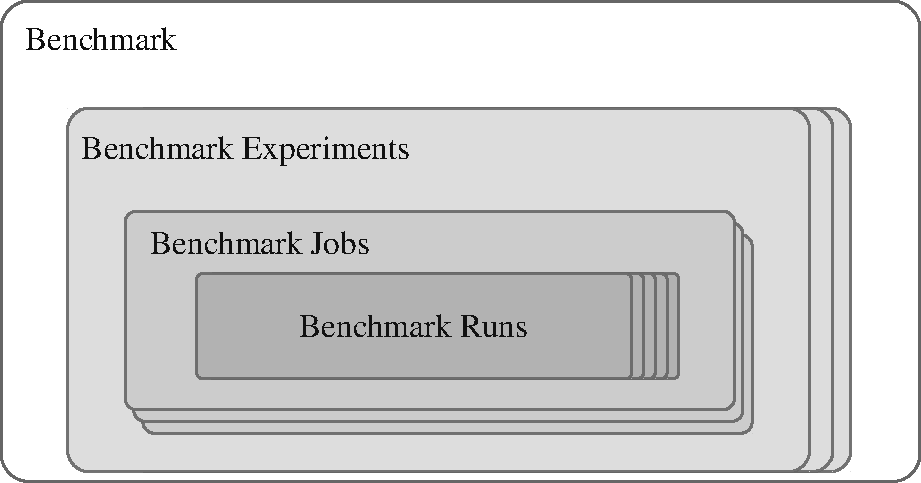
\includegraphics[width=0.6\linewidth]{figures/benchmark-composition.pdf}
	\caption{The composition of a benchmark.}
	\label{fig:benchmark_composition}
\end{figure}

\begin{itemize}
    \item A \textbf{benchmark experiment} addresses a specific performance characteristic of the system-under-test, e.g., the performance of an algorithm, or the weak scalability of a system. Each experiment gathers benchmark results from multiple benchmark jobs to quantify a specific performance characteristic.
    
    \item A \textbf{benchmark job} describes, uniformly across all system-under-tests, the exact job specification of a graph-processing job (See \sref{sec:def:job}). The job specification contains information, e.g., the system-under-test (platform and the environment), the type of algorithm and dataset, and how much resources is used. These information instructs how the system should be configured during the benchmark execution.
    
    \item A \textbf{benchmark run} is a real-world execution of a benchmark job. To gather statistically reliable benchmark results, each benchmark job is repeated multiple times in the form of a benchmark run to mitigate the performance variability during the benchmark execution. 
\end{itemize}




\section{Benchmark Type}
\label{sec:process:type}
The Graphalytics benchmark suite supports four types of benchmark: $\textit{test}$, $\textit{standard}$, $\textit{full}$, and $\textit{custom}$. This section describes the differences and the composition of these four benchmark types.


\subsection{Test Benchmark}
\label{sec:process:type:test}
Running the entire benchmark is very time-consuming. To verify that the cluster environment and all underlying software and hardware stacks are configured properly, the user can choose to first run the test benchmark before starting the actual benchmark. In addition, this can be used to debug a platform driver which is under development.

The test benchmark consists of two experiments which run all six core algorithms on two tiny graphs: ``example-directed" and ``example-undirected", with only one repetition. In total, there are $6 \times 2 \times 1 =  12$ benchmark runs.


\begin{table}[H]
\centering
\begin{tabular*}{0.8\textwidth}{| l@{\extracolsep{\fill}} l |}
\hline
{\bf Experiments}  & \\ \hline
directed ($d$), undirected ($u$) & \\ \hline
\end{tabular*}
\quad 
\begin{tabular*}{0.8\textwidth}{| c@{\extracolsep{\fill}} | c | c | c | c | c | c |}
\hline
{\bf Algorithm} & {\bf Dataset} & {\bf Job} & {\bf Repetition} & {\bf Runs} & {\bf Scale} & {\bf Time-out}    \\ \hline
6 & 2  & 12 & 1 & 12 & $ < 0.5$ & 10 min \\ \hline
\end{tabular*}
\quad 
\begin{tabular*}{0.8\textwidth}{| c@{\extracolsep{\fill}} | c | c | c | c | c | c |}
\hline
{\bf Job} & {\bf BFS} & {\bf WCC} & {\bf PR} & {\bf CDLP} & {\bf LCC} & {\bf SSSP}  \\ 
\hline
{\bf XDIR} & $d$ & $d$ & $d$ & $d$ & $d$ & $d$ \\ \hline
{\bf XUDIR} & $u$ & $u$ & $u$ & $u$ & $u$ & $u$ \\ \hline 
\end{tabular*}
\caption{The benchmark composition of the Test benchmark.}
\label{tab:test_benchmark}
\end{table}


\subsection{Standard Benchmark}
\label{sec:process:type:standard}
Participating in the Graphalytics global competition requires the benchmark to be executed in a standardized format, which is defined as the standard benchmark. The job composition of the standard benchmark should be representative, covering the variability in algorithm complexity and dataset properties that have several impact on the performance of graph processing systems.

The standard benchmark evaluates the system performance with six core algorithms, BFS, WCC, PR, CDLP, LCC, SSSP (See \sref{sec:definition_algorithms}). For each algorithm, five datasets with various of sizes and densities are selected within a target-scale(See \sref{sec:definition_datasets}). Whenever possible, two real-world datasets, two Datagen datasets, and one Graph500 dataset will be included in the dataset selection. If such selection is not possible, e.g., there is a lack of real-world datasets in certain target-scale, or an algorithm requires datasets to be accompanied with edge properties, then additional Datagen datasets will be used to make sure that at least five datasets are available per target-scale.

A standard benchmark can fall into one of the four target-scales, S, M, L, and XL. Each target-scale focuses on processing graphs within certain range of data size, and therefore a corresponding time-out duration has been imposed.  

The standard benchmark (per target-scale) consists of six experiments executing six graph algorithm on five graph graphs, with five repetitions per job. In total, there are $6 \times 5 \times 5 = 150$ benchmark runs.



\begin{table}[H]
\centering
\begin{tabular*}{0.8\textwidth}{| l@{\extracolsep{\fill}} l |}
\hline
{\bf Experiments}  & \\ \hline
BFS ($\textit{bfs}$), WCC ($\textit{wcc}$), PR ($\textit{pr}$), CDLP ($\textit{cdlp}$), LCC ($\textit{lcc}$), SSSP ($\textit{sssp}$) & \\ \hline
\end{tabular*}
\quad 
\begin{tabular*}{0.8\textwidth}{| c@{\extracolsep{\fill}} | c | c | c | c | c | c |}
\hline
{\bf Algorithm} & {\bf Dataset} & {\bf Job} & {\bf Repetition} & {\bf Run}s & {\bf Scale} & {\bf Time-out}    \\ \hline
6 & 6  & 30 & 5 & 150 & $7.5 - 7.9$ & 15 min \\ \hline
\end{tabular*}
\quad 
\begin{tabular*}{0.8\textwidth}{| c@{\extracolsep{\fill}} | c | c | c | c | c | c |}
\hline
{\bf Job} & {\bf BFS} & {\bf WCC} & {\bf PR} & {\bf CDLP} & {\bf LCC} & {\bf SSSP}  \\ 
\hline
DOTA & $\textit{bfs}$ & $\textit{wcc}$ & $\textit{pr}$ & $\textit{cdlp}$ & $\textit{lcc}$ & $\textit{sssp}$   \\ \hline
D7.6 &  &  &  &  &  & $\textit{sssp}$   \\ \hline
D7.7 & $\textit{bfs}$ & $\textit{wcc}$ & $\textit{pr}$ & $\textit{cdlp}$ & $\textit{lcc}$ & $\textit{sssp}$   \\ \hline
D7.8 & $\textit{bfs}$ & $\textit{wcc}$ & $\textit{pr}$ & $\textit{cdlp}$ & $\textit{lcc}$ & $\textit{sssp}$   \\ \hline
D7.9 & $\textit{bfs}$ & $\textit{wcc}$ & $\textit{pr}$ & $\textit{cdlp}$ & $\textit{lcc}$ & $\textit{sssp}$    \\ \hline
G22 & $\textit{bfs}$ & $\textit{wcc}$ & $\textit{pr}$ & $\textit{cdlp}$ & $\textit{lcc}$ &    \\ \hline
\end{tabular*}
\caption{The benchmark composition of the Standard benchmark on target-scale S.}
\label{tab:standard_benchmark_S}
\end{table}


\begin{table}[H]
\centering
\begin{tabular*}{0.8\textwidth}{| l@{\extracolsep{\fill}} l |}
\hline
{\bf Experiments}  & \\ \hline
BFS ($\textit{bfs}$), WCC ($\textit{wcc}$), PR ($\textit{pr}$), CDLP ($\textit{cdlp}$), LCC ($\textit{lcc}$), SSSP ($\textit{sssp}$) & \\ \hline
\end{tabular*}
\quad 
\begin{tabular*}{0.8\textwidth}{| c@{\extracolsep{\fill}} | c | c | c | c | c | c |}
\hline
{\bf Algorithm} & {\bf Dataset} & {\bf Job} & {\bf Repetition} & {\bf Run}s & {\bf Scale} & {\bf Time-out}    \\ \hline
6 & 6  & 30 & 5 & 150 & $8.0 - 8.4$ & 30 min \\ \hline
\end{tabular*}
\quad 
\begin{tabular*}{0.8\textwidth}{| c@{\extracolsep{\fill}} | c | c | c | c | c | c |}
\hline
{\bf Job} & {\bf BFS} & {\bf WCC} & {\bf PR} & {\bf CDLP} & {\bf LCC} & {\bf SSSP}  \\ 
\hline
D8.0 &  &  &  &  &  & $\textit{sssp}$  \\ \hline
D8.1 & $\textit{bfs}$ & $\textit{wcc}$ & $\textit{pr}$ & $\textit{cdlp}$ & $\textit{lcc}$ & $\textit{sssp}$  \\ \hline
D8.2 & $\textit{bfs}$ & $\textit{wcc}$ & $\textit{pr}$ & $\textit{cdlp}$ & $\textit{lcc}$ & $\textit{sssp}$  \\ \hline
D8.3 & $\textit{bfs}$ & $\textit{wcc}$ & $\textit{pr}$ & $\textit{cdlp}$ & $\textit{lcc}$ & $\textit{sssp}$   \\ \hline
D8.4 & $\textit{bfs}$ & $\textit{wcc}$ & $\textit{pr}$ & $\textit{cdlp}$ & $\textit{lcc}$ & $\textit{sssp}$   \\ \hline
G24 & $\textit{bfs}$ & $\textit{wcc}$ & $\textit{pr}$ & $\textit{cdlp}$ & $\textit{lcc}$ &    \\ \hline
\end{tabular*}
\caption{The benchmark composition of the Standard benchmark on target-scale M.}
\label{tab:standard_benchmark_M}
\end{table}






\begin{table}[H]
\centering
\begin{tabular*}{0.8\textwidth}{| l@{\extracolsep{\fill}} l |}
\hline
{\bf Experiments}  & \\ \hline
BFS ($\textit{bfs}$), WCC ($\textit{wcc}$), PR ($\textit{pr}$), CDLP ($\textit{cdlp}$), LCC ($\textit{lcc}$), SSSP ($\textit{sssp}$) & \\ \hline
\end{tabular*}
\quad 
\begin{tabular*}{0.8\textwidth}{| c@{\extracolsep{\fill}} | c | c | c | c | c | c |}
\hline
{\bf Algorithm} & {\bf Dataset} & {\bf Job} & {\bf Repetition} & {\bf Run}s & {\bf Scale} & {\bf Time-out}    \\ \hline
6 & 6  & 30 & 5 & 150 & $8.5 - 8.9$ & 60 min \\ \hline
\end{tabular*}
\quad 
\begin{tabular*}{0.8\textwidth}{| c@{\extracolsep{\fill}} | c | c | c | c | c | c |}
\hline
{\bf Job} & {\bf BFS} & {\bf WCC} & {\bf PR} & {\bf CDLP} & {\bf LCC} & {\bf SSSP}  \\ 
\hline
D8.5 &  &  &  &  &  & $\textit{sssp}$    \\ \hline
D8.6 & $\textit{bfs}$ & $\textit{wcc}$ & $\textit{pr}$ & $\textit{cdlp}$ & $\textit{lcc}$ & $\textit{sssp}$    \\ \hline
D8.7 & $\textit{bfs}$ & $\textit{wcc}$ & $\textit{pr}$ & $\textit{cdlp}$ & $\textit{lcc}$ & $\textit{sssp}$    \\ \hline
D8.8 & $\textit{bfs}$ & $\textit{wcc}$ & $\textit{pr}$ & $\textit{cdlp}$ & $\textit{lcc}$ & $\textit{sssp}$    \\ \hline
D8.9 & $\textit{bfs}$ & $\textit{wcc}$ & $\textit{pr}$ & $\textit{cdlp}$ & $\textit{lcc}$ & $\textit{sssp}$    \\ \hline
G25 & $\textit{bfs}$ & $\textit{wcc}$ & $\textit{pr}$ & $\textit{cdlp}$ & $\textit{lcc}$ &     \\ \hline
\end{tabular*}
\caption{The benchmark composition of the Standard benchmark on target-scale L.}
\label{tab:standard_benchmark_L}
\end{table}


\begin{table}[H]
\centering
\begin{tabular*}{0.8\textwidth}{| l@{\extracolsep{\fill}} l |}
\hline
{\bf Experiments}  & \\ \hline
BFS ($\textit{bfs}$), WCC ($\textit{wcc}$), PR ($\textit{pr}$), CDLP ($\textit{cdlp}$), LCC ($\textit{lcc}$), SSSP ($\textit{sssp}$) & \\ \hline
\end{tabular*}
\quad 
\begin{tabular*}{0.8\textwidth}{| c@{\extracolsep{\fill}} | c | c | c | c | c | c |}
\hline
{\bf Algorithm} & {\bf Dataset} & {\bf Job} & {\bf Repetition} & {\bf Run}s & {\bf Scale} & {\bf Time-out}    \\ \hline
6 & 8 & 30 & 5 & 150 & $9.0 - 9.4$ & 120 min \\ \hline
\end{tabular*}
\quad 
\begin{tabular*}{0.8\textwidth}{| c@{\extracolsep{\fill}} | c | c | c | c | c | c |}
\hline
{\bf Job} & {\bf BFS} & {\bf WCC} & {\bf PR} & {\bf CDLP} & {\bf LCC} & {\bf SSSP}  \\ 
\hline
FSTER  & $\textit{bfs}$ & $\textit{wcc}$ & $\textit{pr}$ & $\textit{cdlp}$ & $\textit{lcc}$ &     \\ \hline
TWIT & $\textit{bfs}$ & $\textit{wcc}$ & $\textit{pr}$ & $\textit{cdlp}$ & $\textit{lcc}$ &     \\\hline
D9.0  &  &  &  &  &  & $\textit{sssp}$   \\ \hline
D9.1  &  &  &  &  &  & $\textit{sssp}$   \\ \hline
D9.2  & $\textit{bfs}$ & $\textit{wcc}$ & $\textit{pr}$ & $\textit{cdlp}$ & $\textit{lcc}$ & $\textit{sssp}$  \\ \hline
D9.3 &  &  &  &  &  & $\textit{sssp}$  \\ \hline
D9.4  & $\textit{bfs}$ & $\textit{wcc}$ & $\textit{pr}$ & $\textit{cdlp}$ & $\textit{lcc}$ & $\textit{sssp}$   \\ \hline
G26  & $\textit{bfs}$ & $\textit{wcc}$ & $\textit{pr}$ & $\textit{cdlp}$ & $\textit{lcc}$ &    \\ \hline
\end{tabular*}
\caption{The benchmark composition of the Standard benchmark on target-scale XL.}
\label{tab:standard_benchmark_XL}
\end{table}




\subsection{Full Benchmark}
\label{sec:process:type:full}
Full benchmark, including new experiment design on quantifying the scalability and robustness of the system-under-test, will be made available in Graphalytics 2.0.

\futureinversion{2.0}{
\paragraph{Scalability Experiments}
For scalable systems, Graphalytics defines two experiments to evaluate the scalability of the system under test. Both experiments must be run with increasing amounts of hardware resources. Which resources are scaled depends on the architecture of the system under test and must be chosen and reported by the benchmark user. Typical examples include scaling the number of machines in a distributed system, scaling the number of processor cores in a parallel machine, or adding GPUs in a heterogeneous system. The system under test as used for the standard experiments is considered the baseline for the scalability experiments. This system is assumed to have N resources for the definition of the scalability experiments.

The strong scalability experiment consists of running BFS and PR on the largest Datagen dataset no larger than the target scale using N, 2N, 4N, 8N, and 16N resources. The weak scalability experiment consists of running BFS and PR on Graph500 datasets of increasing sizes using N, 2N, 4N, 8N, and 16N resources. The largest Graph500 dataset no larger than the target scale must be used for all weak scalability benchmark jobs using N resources, while a Graph500 dataset x times larger is used for a system with xN resources. For example, target scale L requires G25(L) to be run on N resources, G26(XL) on 2N resource, G27(XL) on 4N resources, etc.

For both scalability experiments, all benchmark jobs must be run three times, the makespan and processing time must be reported for each run, and the median processing time must be taken as the processing time of the benchmark job. Per experiment and algorithm the speedup in processing time over using N resources must be reported when using 2N, 4N, 8N, or 16N resources. If any run fails to meet the SLA, no results for the corresponding experiment and algorithm may be reported.
}


\futureinversion{2.0}{
\paragraph{Robustness Experiments}
The robustness of the system under test is evaluated using two experiments targeted at the system's limits through stress testing and at its variability in performance. The workload of the stress test experiments consists of running BFS on all datasets in increasing order of size. The smallest dataset for which the system under test fails the SLA must be reported. If the system under test successfully completes BFS on two synthetic graphs of consecutive scales for a particular dataset generator, successful execution on all smaller graphs for the same generator may be assumed to reduce the number of jobs required to find the system's limit. The workload of the variability experiment consists of running BFS on the largest Datagen dataset no larger than the target scale, which must be repeated ten times. The makespan and processing time must be reported for every run. The variability score of the system under test is the coefficient of variation of the processing times. If any run fails the SLA, no variability score is assigned.
}


\subsection{Custom Benchmark}
\label{sec:process:type:custom}
Custom benchmark, which allows users to define the benchmark composition themselves, will be made available in Graphalytics 2.0.




\section{Benchmark Execution}
\label{sec:process:execution}
The benchmark execution of Graphalytics benchmark suite is illustrated in \fref{fig:benchmark-process}. This section explains how the benchmark suite executes a benchmark with regard to its execution flow, run flow, data flow, metric collection and failure indication.

\begin{figure}[h]
 	\centering
 	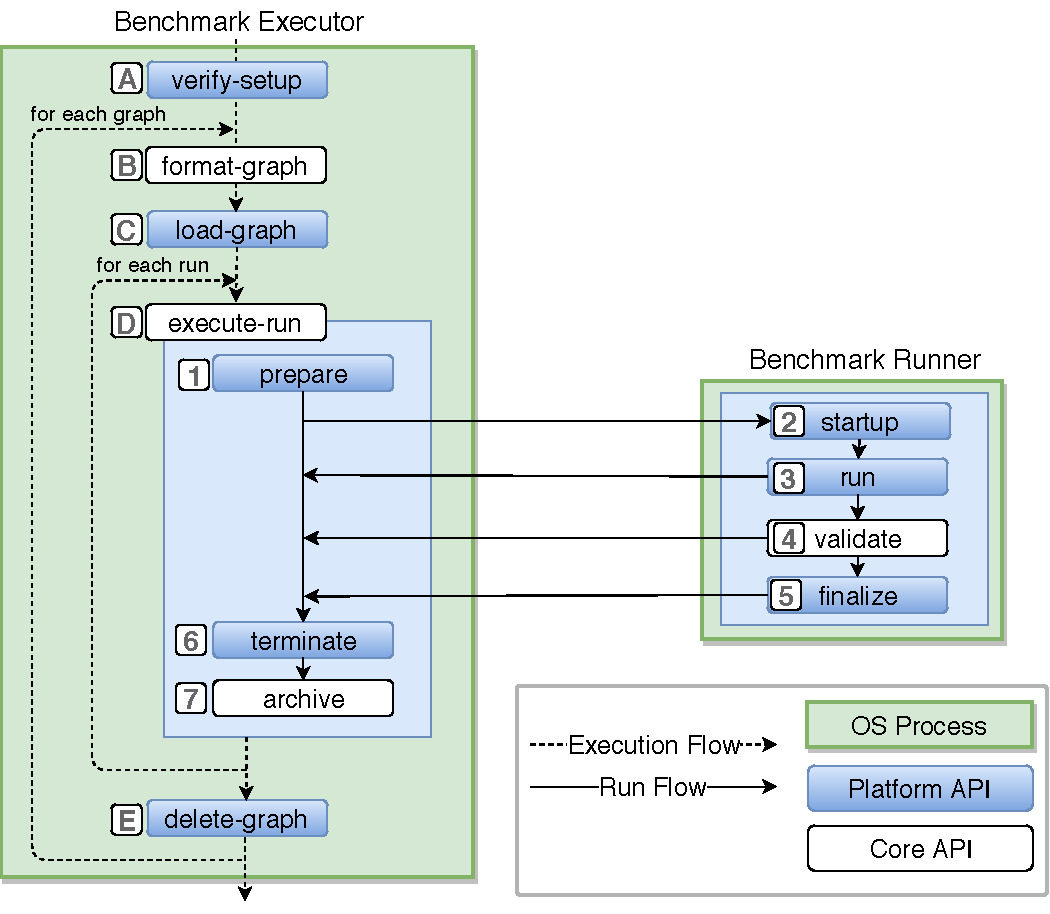
\includegraphics[width=0.9\linewidth]{figures/benchmark_process.pdf}
 	\caption{Benchmark execution in the Graphalytics benchmark suite.}
 	\label{fig:benchmark-process}
\end{figure}


\subsection{Execution Flow}
\label{sec:process:execution:exe_flow}
After a benchmark is loaded, the benchmark suite analyzes the exact composition of the benchmark. Each benchmark consists of a number of benchmark runs, which will be grouped by the graph dataset used by that benchmark run. For each graph dataset, the input data of that dataset will be loaded only once, and be reused for all corresponding benchmarks runs, before finally being removed.

\begin{itemize}
    \item \textbf{[A] Verify-setup}: The benchmark suite verifies that the platform and the environment are properly set up based on the prerequisites defined in the platform driver.
    
    \item \textbf{[B] Format-graph}: The benchmark suite minimizes the ``input data" into ``formatted dataset" (See more in \sref{sec:process:execution:run_flow}) by removing unused vertex and edge properties.
    
    \item \textbf{[C] Load-graph}: The platform converts the ``formatted data" into any platform-specific data format and loads a graph dataset into a storage system, which can be either a local file system, a share file system or a distributed file system. This step corresponds to the ``Loading" step of a graph processing job described in \ref{sec:def:job:operation}.
    
    \item \textbf{[D] Execute-run}: The platform executes a benchmark run with a specific algorithm and dataset (See more details in \sref{sec:process:execution:run_flow}). All benchmark runs using the same input dataset can use the prepared graph dataset during the ``load-graph` step. 
    
    \item \textbf{[E] Delete-graph}: The platform unloads a graph dataset from the storage system, as part of the cleaning up process after all benchmark runs on that graph dataset have been completed.
\end{itemize}

Note that ``load-graph" and ``delete-graph" are platform-specific API, which can be implemented in the platform driver via the ``Platform" interface, whereas  ``execute-run" is a uniform step for all platforms.

\subsection{Run Flow}
\label{sec:process:execution:run_flow}
The execution of each benchmark run consists of seven steps in total, i.e., ``prepare", ``startup", ``run", ``validate", ``finalize", ``terminate", and  ``archive". To ensure the stability, the benchmark suite only prepares for the benchmark, and terminates the benchmark run. Each benchmark run is partially executed in an isolated operating-system process, such that a timed-out job can be terminated properly.

\begin{itemize}
    \item \textbf{Prepare}: The platform requests computation resources from the cluster environment and makes the background applications ready.
    
    \item \textbf{Startup}: The platform configures the benchmark run with regard to real-time cluster deployment information, e.g., input directory, output directory and log directory.
    
    \item \textbf{Run}: The platform runs a graph-processing job as defined in the benchmark run. The graph-processing job must complete within the time-out duration, or the benchmark run will fail. This step corresponds to the ``Running" step of a graph processing job described in \ref{sec:def:job:operation}.
    
    \item \textbf{Validate}: The benchmark suite validates the platform output with the validation data. The system-under-test must succeed in this step, or the benchmark run will fail.
    
    \item \textbf{Finalize}: The platform reports the benchmark information and makes the environment ready for the next benchmark run.
    
    \item \textbf{Terminate}: The platform forcibly stops the benchmark job and clean up the environment, given that the time-out has been reached. 
    
    \item \textbf{Archive}: The benchmark suite archives the benchmark results, gathering information regarding performance metrics and failure indications.
\end{itemize}

Note that ``prepare", ``startup", ``run", ``finalize", ``terminate", and ``archive" are platform-specific API, which can be implemented in the platform driver via the ``Platform" interface, whereas ``archive" is a uniform step for all platforms. 


\subsection{Data Flow}
\label{sec:process:execution:data_flow}
The graph datasets go through a series of execution steps during the benchmark execution, and in the process of which the format, the representation, and the content of the graph dataset change accordingly.

For each graph, the input datasets and the validation datasets are publicly available benchmark resources.

\begin{itemize} 
    \item \textbf{Input data}: The ``input data" consists of a vertex file and edge file in EVLP format, as defined in \sref{sec:data:representation}.
    \item \textbf{Validation data}: The ``validation data" consists of correct outputs for all six core algorithm, as defined in \sref{sec:definitions_validation}.
\end{itemize}

The input dataset can be converted into the following format during the benchmark.

\begin{itemize}
    \item \textbf{Formatted data}: The ``input data" can plausibly contain dozens of vertex and edge properties. During the ``load-graph" step, the benchmark suite identifies for each algorithms which properties are needed and which are not, and minimizes the ``input data" into the ``formatted data". The ``formatted data" is cached in the storage system for future uses. 
    \item \textbf{Loaded data}: The minimized ``formatted data" is loaded into a storage system during the ``load-graph" step, which can either be a local file system, a share file system or a distributed file system.
    \item \textbf{Output data}: The ``output data" is the output of a graph-processing job being benchmarked during the ``process" step. The ``output data" is compared to the ``validation data" to ensure the correctness of the benchmark execution.
\end{itemize}



\subsection{Failure Indication}
\label{sec:process:execution:failure}
Failures can occur during the benchmark for many reasons. The benchmark suite logs the benchmark execution and classifies the type of failures.


\begin{itemize}
    \item \textbf{DAT}: ``Data failure" occurs when the ``format-graph`` step fails to generate ``formatted-graph``, or the ``load-graph" step fails to complete correctly. For example, ``input graph" can be missing or simply be misplaced, or alternatively the conversion from ``input-graph" to ``formatted-graph" could be prematurely interrupted, which leads to data corruption.
    
    \item \textbf{INI}: ``Initialization failure" occurs when the platform fails to properly make the environment ready for the benchmark during the ``prepare" or ``startup" step. For example, the deployment system may fail to allocate the cluster resources needed.
    
    \item \textbf{EXE}: ``Execution failure" occurs when the execution of the benchmark run fails to complete during the ``run" step.
    
    \item \textbf{TIM}: ``Time-out failure" occurs when the pre-defined time-out duration is reached during the ``run" step.

    \item \textbf{COM}: ``Completion failure" occurs when output results are incomplete or cannot be found at all. For example, outputs from some compute nodes can be fetched incorrectly.
    
    \item \textbf{VAL}: ``Validation failure" occurs when the ``output data" is returned by the system, but fails the validation during the ``validate" step.
    
    \item \textbf{MET}: ``Metric failure" occurs when the compulsory performance metrics are missing during the ``archive" step. For example, the log files containing the information can be non-existing or corrupted.
\end{itemize}










\section{Benchmark Result}

\futureinversion{1.0}{The benchmark result will be updated according to the implementation.} A complete result for the Graphalytics benchmark includes at least the following information: 

\begin{enumerate}
	\item Target scale (T).
	\item Environment specification, including number and type of CPUs, amount of memory, type of network, etc.
	\item Versions of the platform and Graphalytics drivers used in the experiments.
	\item Any non-default configuration options for the platform required to reproduce the system under test.
	\item For every benchmark job:
		\begin{enumerate}
			\item Job specification, i.e., dataset and algorithm.
			\item For every platform run, report the measured processing time, makespan, and whether the run breached the Graphalytics SLA.
			\item (optional) {\tt Granula} archives for each platform run, enabling deep inspection, visualization, modeling, and sharing of performance data.  
		\end{enumerate}
		
\futureinversion{2.0}{
	\item If scalability experiments are performed:
		\begin{enumerate}
			\item Definition of the hardware resources that were scaled up for each scalability experiment.
			\item For every benchmark job corresponding to a scalability experiment, include the resource scale (i.e., 1, 2, 4, 8, or 16).
		\end{enumerate}
}

\futureinversion{2.0}{
	\item 
	If robustness experiments are performed:
		\begin{enumerate}
			\item Summary of the results for every benchmark job.
		\end{enumerate}	
}

\end{enumerate}
Future versions of the benchmark specification will include a Full Disclosure Report template and a process for submitting official Graphalytics results. A sample data format can be found in Appendix~\ref{chap:data-format}.

